\section{Описание задания и программной реализации}
	\subsection{Краткое описание задания}
		Задание можно разбить на 4 этапа:
		\begin{enumerate}
			\item Generate - генерация графа/портрета по тестовой сетке. По двумерной неструктурированной смешанной сетке, состоящей из треугольников и четырёхугольников генерируется портрет разреженной матрицы смежности графа, дополненный главной диагональю в формате CSR.
			\item Fill - заполнение матрицы и вектора правой части по заданному портрету.
			\item Solve - решение СЛАУ с полученной матрицей. Так как матрица, полученная на предыдущем этапе, симметричная, то используется метод сопряженных градиентов с предобуславливателем Якоби.
			\item Report - проверка корректности и выдача измерений. Проверка, что невязка системы после работы решателя удовлетворяет заданной точности, выдача значения невязки и печать таблицы таймирования всех предыдущих этапов.

		\end{enumerate}

	\subsection{Краткое описание программной реализации}
		Сначала в функции \textit{main} происходит считывание данных командной строки, проверка их корректности и выдача диагностики. Параметры программы: \textit{Nx}, \textit{Ny}, \textit{K1}, \textit{K2}. Их значение хорошо поясняет рисунок \ref{param}. В случае параллельной реализации после них ещё идёт количество используемых нитей. А в самом конце может быть необязательный аргумент включающий отладочную печать.
			\begin{figure}[H]
		        \centering
		        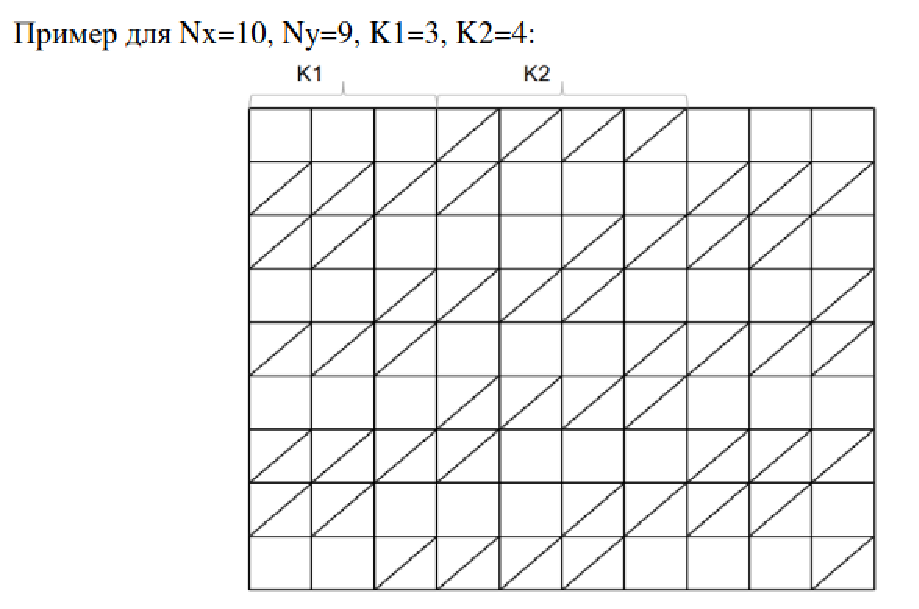
\includegraphics[width=0.5\textwidth]{./images/param}
		        \caption{Параметры командной строки}
		        \label{param}
		    \end{figure}


	\begin{lstlisting}[numbersep=10pt, language=C++, caption=\textbf{Реализованные функции}]
// Inner product of two vectors vec_1 ans vec_2
double dotKernel(const std::vector<double>& vec_1, const std::vector<double>& vec_2);

// Linear combination of two vectors x = a * x + b * y
void axpbyKernel(const double a, std::vector<double>& x,
	             const double b, const std::vector<double>& y);

// Matrix vector product with sparse matrix. row_ptr, col_ptr - CSR representation, res = Matrix * vec
void SpMVKernel(const std::vector<double>& matrix, const std::vector<int>& row_ptr,
	            const std::vector<int>& col_ptr, const std::vector<double>& vec,
	            std::vector<double>& res);

// Compution, how many cells with obliques line before cell with index cell_idx, K1, K2 - parameters that determine the distribution of oblique lines
int obliquesBefore(const int K1, const int K2, const int cell_idx);

// Determines whether a cell with the cell_idx index contains oblique line,  K1, K2 - parameters that determine the distribution of oblique lines
bool hasOblique(const int K1, const int K2, const int cell_idx);

// Function corresponds to the first stage of the task. Nx, Ny, K1, K2 - determine the configuration of a two-dimensional grid, row_ptr, col_ptr - CSR representation
void generate(const int Nx, const int Ny, const int K1, const int K2, std::vector<int>& row_ptr, std::vector<int>& col_ptr);

// Function corresponds to the second stage of the task. Nx, Ny - determine grid size, row_ptr, col_ptr - CSR representation, A_arr, b_vec - fillable matrix and vector
void fill(const int Nx, const int Ny,
	      const std::vector<int>& row_ptr, const std::vector<int>& col_ptr,
	      std::vector<double>& A_arr, std::vector<double>& b_vec);

// Function corresponds to the third stage of the task. A_arr, b_vec - initial data for solving systems of linear equations, row_ptr, col_ptr - CSR representation, x_vec - equations solution, TOL - relative error of the solution
void Solve(const std::vector<double>& A_arr, const std::vector<double>& b_vec,
	       const std::vector<int>& row_ptr, const std::vector<int>& col_ptr,
	       std::vector<double>& x_vec, const double TOL = 1e-4);
	\end{lstlisting}
\section{Исследование производительности}
	\subsection{Характеристики вычислительной системы}
	Тестирования программы проводились на вычислительном комплексе \textit{IBM Polus}. Polus - параллельная вычислительная система, состоящая из 5 вычислительных узлов. Каждый узел оборудован двумя десятиядерными процессорами \textit{IBM Power 8}, каждое ядро которого имеет 8 потоков, 256-ю GB оперативной памяти. Производительность кластера (TFlop/s): 55,84 (пиковая), 40,39 (Linpack).
	\subsection{Результаты измерений производительности}
			\begin{tabular}{|c||c|c|c|c|c|c|}
				\hline
				\multirow{2}{*}{N} &  \multirow{2}{*}{Generation} & \multirow{2}{*}{Filling} & Dot & Axpby & SpMV          & \multirow{2}{*}{Memory} \\ \cline{4-6}
				                   &                              &                         & \multicolumn{3}{c|}{Solver}  &                         \\ \hline
                \multirow{2}{*}{10000} & \multirow{2}{*}{0.000106} & \multirow{2}{*}{0.002573} & 0.000472 & 0.000278 & 0.001478              & \multirow{2}{*}{1.37} \\ \cline{4-6}
                                       &                     &                    & \multicolumn{3}{c|}{0.002410} &               \\ \hline
                \multirow{2}{*}{100000} &  \multirow{2}{*}{0.000976} & \multirow{2}{*}{0.029809} & 0.004713 & 0.003035 & 0.014737 & \multirow{2}{*}{12.65} \\ \cline{4-6}
                                      &                     &                     & \multicolumn{3}{c|}{0.023898} &  \\ \hline
                \multirow{2}{*}{100000} &  \multirow{2}{*}{0.008699} & \multirow{2}{*}{0.298622} & 0.052439 & 0.034897 & 0.161633 & \multirow{2}{*}{124.66} \\ \cline{4-6}
                                       &                     &                    & \multicolumn{3}{c|}{0.261804} &  \\ \hline
                \multirow{2}{*}{1000000} &  \multirow{2}{*}{0.086874} & \multirow{2}{*}{3.014130} & 0.517145 & 0.326723 & 1.640600 & \multirow{2}{*}{1224.79} \\ \cline{4-6}
                                       &                     &                    & \multicolumn{3}{c|}{2.622970} &  \\ \hline


				
			\end{tabular}
		\subsubsection{Последовательная производительность}
		\subsubsection{Параллельное ускорение}
\section{Анализ полученных результатов}

\clearpage
%\newpage